\documentclass[paper=a4,11pt,titlepage,twoside=true,headings=normal,numbers=noenddot,captions=tableabove,listof=totoc,index=totoc,bibliography=totoc]{scrreprt}
%\usepackage{amsmath} % abgesetzte Formeln zentriert in der Zeile
%\usepackage[fleqn,intlimits]{amsmath} % [fleqn] abgesetzte Formeln mit festem Abstand zum linken Rand
\usepackage[reqno,intlimits]{amsmath} % [reqno] um die gleichungsnummerierung rechts zu haben
% intlimits: Grenzen für Integrale unterhalb und oberhalb des Zeichens
\usepackage{amssymb}
\usepackage{array}
%\usepackage[ngerman]{babel}
%\usepackage[ngerman]{varioref}
\usepackage[english]{babel}
\usepackage[english]{varioref}
\usepackage[T1]{fontenc} 
\usepackage[utf8]{inputenc}
%---------------------------
\usepackage{booktabs}
\usepackage{calc}
\usepackage{cancel}
\usepackage[labelfont={footnotesize,sf,bf},textfont={footnotesize,sf}]{caption} %Format (Textgröße, Textform) für Bildtext 
%normalsize
%scriptsize
% sc --> smallcaps
% bf --> bold face
% sf --> sans serif
%\usepackage{cite} %inkompatibel mit biblatex
\usepackage[table]{xcolor}
%\usepackage{colortbl}
\usepackage[right]{eurosym}
%\usepackage{caption2} %nicht zusammen mit sidecap
%\usepackage{exscale}
\usepackage{ellipsis}
\usepackage{graphicx}
\usepackage{float}
%\usepackage{floatflt}
%----------------------------------------
\usepackage{gensymb} %-----------
%\usepackage{helvet}
\usepackage{csquotes}
\usepackage{listings}
\usepackage{longtable}
\usepackage{lastpage}  %----------
\usepackage{lscape}
\usepackage{lmodern}  %-- Silbentrennung
%\usepackage{mathpazo} % andere mathematische Symbol
\usepackage{makeidx}
%\usepackage{minitoc}
\usepackage{multirow}
\usepackage{multicol}
%\usepackage[intoc]{nomencl}   % zwei Spalten beim Formelzeichenverzeichnis
%\usepackage[german,intoc]{nomentbl} %vier Spalten bei Formelzeichenverzeichnis
\usepackage[english,intoc]{nomentbl} %vier Spalten bei Formelzeichenverzeichnis
\usepackage{nicefrac} %----
%\usepackage{picins} %----------
\usepackage{paralist} %--------
\usepackage{parallel}  %----------
\usepackage{pdfpages} %-------
% Define user colors using the RGB model
%\usepackage{colortbl}
%\definecolor{dunkelgrau}{rgb}{0.8,0.8,0.8}
%\definecolor{hellgrau}{rgb}{0.95,0.95,0.95}
%\usepackage{pgfplots}
\usepackage[figuresright]{rotating} 
\usepackage{scrlayer-scrpage}
%\usepackage[innercaption]{sidecap} %Beschriftung neben Bild, Tabelle, Mittelbach S333 %----------
%\usepackage{sistyle}
%\usepackage[locale=DE]{siunitx} %nicht zusammen mit sistyle %---------
\usepackage[locale=DE,per-mode=fraction,parse-numbers=false]{siunitx} %nicht zusammen mit sistyle %---------
\usepackage[font={scriptsize,sl},captionskip=3pt]{subfig} % für die Unterbilder %---------
\usepackage{shortvrb}
\usepackage{tablefootnote}
\usepackage{tabularx}
\usepackage{tabulary}
\usepackage{textcomp}
\usepackage{tocbasic}
%\usepackage{tikz}
\usepackage{times} 
\usepackage{units} %----------
\usepackage{url}
\usepackage{wrapfig} %----------
\usepackage{xr-hyper}
\usepackage{arydshln} %für \hdashline[5pt/2pt] % muss am Ende stehen, sonst gibt es Probleme mit xcolor
\usepackage{hyperref} % muss am Schluss stehen
\hypersetup{linkcolor={0 1 1}, linkbordercolor={1 1 1}, citebordercolor={1 1 1}} % setzt Linkboxen auf Farbe "`weiß"'
%\usepackage{bm}
%\usepackage[toc,symbols]{glossaries} %---------- muss nach hyperref stehen
\usepackage[nonumberlist, acronym, toc, section]{glossaries} % muss nach hypersetup stehen
%----------------
%\usepackage{romannum} % Seitenzahlen in römischen Ziffern
%\usepackage{adjustbox}
\usepackage{scrhack}
\usepackage[style=phys, citestyle=numeric, backend=biber]{biblatex}
\usepackage[useregional]{datetime2}
\usepackage{cleveref} % löscht labels!!!!!!!!!! <--- warum? habs trotzdem eingefügt weil es die referencen nice macht ohne newcommands dafür zu brauchen. außerdem steht intellisense drauf ;)
\usepackage{isotope} % um chemische gleichungen hübscher darstellen zu können
\usepackage{framed} % um dinge zu umrahmen
%-------------------------
 %\renewcommand{\captionlabelfont}{\sffamily} %für "Abbildung" und "Tabelle"
 %\renewcommand{\captionfont}{\sffamily\small} %für den Text der Bildunterschriften
%  \renewcommand{\captionlabelfont}{\sffamily} 
%  \renewcommand{\captionfont}{\sffamily} %\renewcommand{\normalfont}{\sffamily} %für die Überschriften
% Fettdruck der Bezeichnung Abbildung, Tabelle
%\renewcommand{\captionlabelfont}{\bfseries}
%---------------------------------------------
%------------------ Schrifttyp in der Kopf- und Fusszeilen
\setkomafont{pageheadfoot}{\footnotesize\sffamily}
%---------------------------------------------------
%Ändern der Abbildung- und Tabellenbezeichnung (Niedermair S.157)
%_____________________________________________
\addto\captionsngerman{\renewcommand\figurename{Abb.}}
\addto\captionsngerman{\renewcommand\tablename{Tab.}}
\renewcommand\listfigurename{Abbildungen}
%_______________________________
%Betrag eines Wertes
\newcommand{\abs}[1]{\lvert #1 \rvert} 
%---------------------------------------------
\newcommand{\absatz}[1]{\textbf{\textsc{#1}}} %siehe Mittelbach S. 876ff
%----------------------------
%\newcommand{\absatz}{\par \medskip}
%______________________________
%\newcommand{\anhang}[1]{Anhang \ref{#1}, Seite \pageref{#1}}
\newcommand{\anhang}[1]{Anhang \vref{#1}}
%________________________________
\newcommand{\aufgabe}{\stepcounter{plus} Aufgabe \arabic{plus}}
%______________________________________
%compactitem
\newcommand{\bci}{\begin{compactitem}}
\newcommand{\eci}{\end{compactitem}}
%______________________________________
%
\newcommand{\bi}{\begin{itemize}}
\newcommand{\ei}{\end{itemize}}
%______________________________________
%compactenumerate
\newcommand{\bce}{\begin{compactenum}}
\newcommand{\ece}{\end{compactenum}}
%_____________________________________
%begin equation
\newcommand{\be}{\begin{equation}}
\newcommand{\ee}{\end{equation}}
%_____________________________________
%begin equation ohne Formelnummer
\newcommand{\ben}{\begin{equation*}}
\newcommand{\een}{\end{equation*}}
%_____________________________________
%begin align ohne Formelnummer
\newcommand{\ban}{\begin{align*}}
\newcommand{\ean}{\end{align*}}
%_____________________________________
%begin align
\newcommand{\ba}{\begin{align} }
\newcommand{\ea}{\end{align}}
%_____________________________________
%minpage
\newcommand{\bmp}{\begin{minipage}[t]{.47\linewidth}}
\newcommand{\emp}{\end{minipage}}
%_____________________________
%  dB
\newcommand{\db}{dB}
%  dB(A)
\newcommand{\dba}{ dB(A) }
%  dB(A) für Satzende
\newcommand{\dbap}{ dB(A)}
%_________________________________
\newcommand{\bzw}{bzw.\,}
%_______________________________
\newcommand{\dif}{\mathrm{d}}
%________________________________
% neuer Zähler
\newcounter{plus}
\setcounter{plus}{0}
%______________________________
%Für das Formelverzeichnis _____________________ Formelverzeichis ____
% Befehl umbenennen in fz
\let\fz\nomenclature
% Deutsche Überschrift
\renewcommand{\nomname}{Formelzeichen}
% Punkte zw. Abkürzung und Erklärung
\setlength{\nomlabelwidth}{.20\hsize}
\renewcommand{\nomlabel}[1]{#1 \dotfill}
% Zeilenabstände verkleinern
\setlength{\nomitemsep}{-\parsep}
%_____________________________
\newcommand{\bild}[1]{Abb. \vref{#1}}
\newcommand{\sbild}[1]{siehe Abb. \vref{#1}}
\newcommand{\bilder}[2]{Abb. \vrefrange{#1}{#2}}
\newcommand{\bildseite}[1]{Abb. \vref{#1}} % erzeugt "`Abb. nn auf Seite nn
\newcommand{\tabelle}[1]{Tab. \vref{#1}}
\newcommand{\tabellenseite}[1]{Tab. \vref{#1}} % erzeugt "`Tab. nn auf Seite nn
% für \vref ist usepackage[german]{varioref} einzufügen
%_-------------------------------- Freiraum
\newcommand{\freiraum}[1]{\begin{figure}[H]\vspace{#1\textheight}\end{figure}}
%_____________________________
% Gleichung
\newcommand{\gl}[1]{Gl.\,(\ref{#1})}
\newcommand{\sgl}[1]{siehe Gl.\,(\ref{#1})}
\newcommand{\glbereich}[2]{Gl. \vrefrange[]{#1}{#2}}
%_____________________________
% Grad Celsius
\newcommand{\grad}{\,\degC}
\newcommand{\gradC}{\,\degree}
%______________________________________
% Großbuchstaben als Indizes kleiner schreiben; spezielle im Mathemodus
\newcommand{\klein}[1]{\scriptscriptstyle{#1}}% Fettdruck der Bezeichnung 
%______________________________
%% Kasten
\newcommand{\kasten}{\fbox{\rule{0.0pt}{10pt}{{ } } }}
%______________________________
%\newcommand{\kapitel}[1]{Kapitel \ref{#1}, Seite \pageref{#1}}
\newcommand{\kapitel}[1]{Kapitel \vref{#1}}
%_____________________________
%  LAeq für den äquivalenten Dauerschallpegel
\newcommand{\laeq}{ $L_{Aeq}$ }
%  LAeq für den äquivalenten Dauerschallpegel am Satzende
\newcommand{\laeqp}{ $L_{Aeq}$}
%_________________________________
%   Linie zeichnen
\newcommand{\linie}{\rule{0.5\textwidth}{0.1pt}}
%---------------------- LaTeX
\newcommand{\lt}{\LaTeX\,\,}
%----------------------------
\newcommand{\nl}{\newline}
%__________________________________
%  multicolumn für Tabellen
\newcommand{\mc}{\multicolumn}
%% \mc{1}{c}{Text}
%_________________________________
%    Parallel
\newcommand{\pl}[1]{\ParallelLText{#1}}
\newcommand{\pr}[1]{\ParallelRText{#1}}
\newcommand{\pp}{\ParallelPar}
%------------ rot unterstrichen
\newcommand{\rotunterstrichen}[1]{\textcolor{red}{\underline{\textcolor{black}{#1}}}}
%________________ Realteil
\newcommand{\real}[1]{\text{Re}\left\{#1\right\}}
%________________________________--
\newcommand{\seite}[1]{Seite \pageref{#1}}
\newcommand{\seiten}[2]{\vpagerefrange{#1}{#2}}
%----------------------------
%        TEXT Rot
\newcommand{\textrot}[1]{\textcolor{red}{#1}}
%______________________________
%Abkürzung für \multicolumn
\newcommand{\tab}[2]{\multicolumn{1}{#1}{#2}}
%_____________________________________
% doppelt unterstreichen
\newcommand{\unterstreichen}[1]{\underline{\underline{#1}}}
% einfach unterstreichen
\newcommand{\ul}[1]{\underline{#1}}
%______________________________
%kurze Verbatimausgabe
%\MakeShortVerb{\|} %mittelbach S.160 mit \usepackage{shortvrb}
%_______________________________________
% vspace
\newcommand{\vsf}{\vspace{5pt}}
%_________________________________
\newcommand{\zb}{z.B.\,}
\newcommand{\idr}{i.d.R.\,}
%_______________________________
% Zähler-einfach
\newcounter{req}
\newcommand{\zaehler}[1]{\refstepcounter{req}{#1} \thereq}
%% Beispielaufzählung \zaehler{Beispiel}\\
%_____________________________________
\creflabelformat{equation}{\textup{#2#1#3}}
\hypersetup{colorlinks=false, urlcolor=blue, linkcolor=blue, citecolor=black}
\setlength{\voffset}{-2.532 cm}
\setlength{\hoffset}{-1.57 cm}
% \setlength{\topmargin}{2.0 cm} \setlength{\topskip}{0.1 cm}
\setlength{\topmargin}{1.5 cm}
\setlength{\topskip}{0.1 cm}
\setlength{\evensidemargin}{1.5 cm}
\setlength{\oddsidemargin}{1.5 cm}
\setlength{\textwidth}{16.5 cm}
\setlength{\footskip}{40pt}
\setlength{\textheight}{24.5cm}
% \setlength{\textheight}{23.5 cm}
\setcounter{page}{1}
\setlength{\parindent}{0mm}
\setlength{\headsep}{20pt}
\setlength{\abovedisplayskip}{10pt}
\setlength{\belowdisplayskip}{10pt}
\setlength{\abovedisplayshortskip}{10pt}
\setlength{\belowdisplayshortskip}{10pt}
%----------------------------------------------------------------------
% Linien in der Kopf- und Fußzeile
%\renewcommand{\headrulewidth}{0.0pt}   %Linie in der Kopfzeile mit 0.0pt keine Linie
%%\renewcommand{\footrulewidth}{0.0pt}   %Linie in der Fußzeile mit 0.0 pt keine Linie
%\renewcommand{\headrulewidth}{0.2pt}   %Linie in der Kopfzeile mit 0.0pt keine Linie
%\renewcommand{\footrulewidth}{0.2pt}   %Linie in der Fußzeile mit 0.0 pt keine Linie
%------------------------------------------------------------------------
%\renewcommand{\normalfont}{\sffamily} %für die Überschriften
%\renewcommand{\chaptermark}[1]{\markboth{\chaptername\ \thechapter #1}{}}
%\renewcommand{\sectionmark}[1]{\markright{\thesection\ #1}}
% \rfoot{\leftmark\\\rightmark}

%Definitionen für Kopfzeile
% bei documentclass {report} hat der Eintrag für die [gerade Seite] keine Wirkung
%-------------------------------------------------------------
%%
%Einstellungen für Kopf- und Fusszeilen mit dem KOMA-Skript und \usepackage{scrpage2}
\pagestyle{scrheadings}
%\pagestyle{scrplain}
% le --> links, gerade Seite
% ce --> mittig, gerade Seite
% re --> rechts, gerade Seite
% lo --> links, ungerade Seite
% co --> mittig, ungerade Seite
% ro --> rechts, ungerade Seite
%---------------------------------------------
% Löschen aller Einträge
%\clearscrheadings
% \automark[section]{subsection}
% \pagemark --> Seitenzahl
% \automark --> Kapitelüberschriften
% \leftmark --> ??
% \rightmark --> ??
%::::::::::::::::::::::::::::::::::: Kopfzeile
% Kopfzeile gerade Seite
\automark[chapter]{chapter}
\lehead[]{\titelkopfzeilelinkseven}
\cehead[]{\titelkopfzeilemitteeven}
\rehead[]{\titelkopfzeilerechtseven}
% Kopfzeile ungerade Seite
\lohead[]{\titelkopfzeilelinksodd}
\cohead[]{\titelkopfzeilemitteodd}
\rohead[]{\titelkopfzeilerechtsodd}
% Linie in der Kopfzeile
%\setheadtopline{0.2pt} % obere Linie in der Kopfzeile; nur bei scrartcl
\setheadsepline{0.4pt} % untere Linie in der Kopfzeile; nur bei scrartcl
% Linie in der Fusszeile
%::::::::::::::::::::::::::::::::::: Fußzeile
% Fusszeile gerade Seite[plain-style]{scrheadings-style}
\lefoot[]{\titelfusszeilelinkseven} 
\cefoot[]{\titelfusszeilemitteeven}
\refoot[]{\titelfusszeilerechtseven}
% Fusszeile ungerade Seite
\lofoot[]{\titelfusszeilelinksodd}
\cofoot[]{\titelfusszeilemitteodd}
\rofoot[]{\titelfusszeilerechtsodd}
%\rofoot[\thepage ]{\thepage}
%\setfoottopline{0.2pt} % obere Linie in der Kopfzeile; nur bei scrartcl
\setfootsepline{0.4pt} % untere Linie in der Kopfzeile; nur bei scrartcl

% le --> links, gerade Seite
% ce --> mittig, gerade Seite
% re --> rechts, gerade Seite
% lo --> links, ungerade Seite
% co --> mittig, ungerade Seite
% ro --> rechts, ungerade Seite
% even --> gerade Seite
% odd --> ungerade Seite
%----------------------------------------- Kopfzeilentext
 \newcommand{\titelkopfzeilemitteeven}{}
 \newcommand{\titelkopfzeilemitteodd}{}
 \newcommand{\titelkopfzeilelinkseven}{Hochschule RheinMain}
 \newcommand{\titelkopfzeilelinksodd}{}
 \newcommand{\titelkopfzeilerechtseven}{}
 \newcommand{\titelkopfzeilerechtsodd}{Hochschule RheinMain}
 %----------------------------------------- Fußzeilentext
 \newcommand{\titelfusszeilemitteeven}{}
 \newcommand{\titelfusszeilemitteodd}{}
 \newcommand{\titelfusszeilerechtseven}{Studienbereich Angewandte Physik \& Medizintechnik}
 \newcommand{\titelfusszeilerechtsodd}{\thepage \hspace{0.5mm} von \pageref{LastPage}}
 \newcommand{\titelfusszeilelinkseven}{\thepage \hspace{0.5mm} von \pageref{LastPage}}
 \newcommand{\titelfusszeilelinksodd}{Studienbereich Angewandte Physik \& Medizintechnik}
\newcommand{\titelLV}{Physics Lab 3}
%---------------------------- VARIABLEN festlegen ------------------
%----------- Pro Versuch zu ändernde Angaben -----------------------
\newcommand{\versuch}{3} % Versuchsnummer einfügen
\newcommand{\untertitelb}{Torsional Pendulum} % Titel des Versuchs einfügen
\newcommand{\datumLV}{17.11.2020} % Datum einfügen
\newcommand{\deadline}{1.12.2020} % Abgabedatum ist der 1.12.2020
\newcommand{\dateLVa}{Dezember 15, 2020}
\newcommand{\dateLVb}{January 5, 2021}
%----------- TITEL
\newcommand{\untertitela}{Experiment P3-3}
% -------- Student 1
\newcommand{\nameA}{Hunter, Dennis}
% --------- Student 2
\newcommand{\nameB}{Kreß, Sebastian}
% --------- Student 3, falls vorhanden
\newcommand{\nameC}{Ünlü, Cihan}
%::::::::::::::::::::::::::::::::::
%\renewcommand\USenglishtoday
\DeclareNameAlias{author}{last-first}
\DeclareNameAlias{editor}{last-first}
\DeclareNameAlias{translator}{last-first}
\addbibresource{quellen.bib}
\begin{document}%\selectlanguage{USenglish}
%-----------------------------------------------------------------
\begin{titlepage} 
	\newcommand{\HRule}{\rule{\linewidth}{0.5mm}} 	
	\centering
	\textsc{\Large Hochschule RheinMain \\
		
\includegraphics[width=0.15\textwidth]{logo-hsrm}\\[1cm]}
%	\textsc{\Large Hochschule RheinMain}\\[1cm]
	\textsc{\LARGE \titelLV}\\[0.5cm]
		\HRule\\[0.4cm]
	{\huge\bfseries \untertitela}\\[0.4cm] % Title des Dokuments
	{\huge\bfseries \untertitelb}\\[0.4cm] % Title des Dokuments
		\HRule\\[1.5cm]
%-------------------
%\begin{flushleft}
	\begin{minipage}{0.4\textwidth}
%	\begin{flushleft}
%\centering
		\large
		\textit{\underline{Authors}}\\[0.5cm]
		\textsc{\nameA}\\[0.5cm]
		\textsc{\nameB}\\[0.5cm]
		\textsc{\nameC}\\[0.5cm]
		%\textsc{\nameC}\\[0.5cm] 
%	\end{flushleft}
\end{minipage}
%------------------------------------
\vfill\vfill\vfill 
%\textsc{\Large Fachbereich Ingenieurwissenschaften}\\[0.5cm]
\textsc{\Large Department of Engineering}\\[0.5cm]
%\textsc{\large Studienbereich Angewandte Physik \& Medizintechnik}\\[0.5cm]
\textsc{\large Applied Physics \& Medical Technology}\\[0.5cm]
\vfill
\begin{tabular}{ll}
	Date of experiment:\hspace{0.4cm} &{\large\dateLVa}\\
	Date of submission:\hspace{0.4cm} &{\large\today} 
\end{tabular}
\end{titlepage}

%-----------------------------------------------------
\tableofcontents
\newpage
%--------------------
\chapter{Introduction}
%
\section{Terms and Definitions}
    \subsection*{Free Harmonic and Damped Oscillation}
        If a system capable of oscillation is deflected out of its equilibrium position and is experiencing a restoring force
        proportional to its deflection this system is called a \textit{harmonic oscillator}. If a dampening force such as friction
        is introduced, the system no longer oscillates freely but rather damped.\par
        Both, damped and harmonic oscillations are considered \textit{free} if there is no continuous, the oscillation driving
        stimulus present.
        %
    \subsection*{Natural Angular Frequency of a Harmonic Oscillation}
        %
        Depending on the very characteristics of the given system it will oscillate at a distinct frequency - the natural angular
        frequency \( \omega_0 \).
    \subsection*{Differential Equation of the Damped Harmonic Oscillation}
        \begin{equation}
            I \ddot{\varphi} = -D\varphi -\rho\dot{\varphi}+M\cos(\omega t)
        \end{equation}
    \subsection*{Damping cases}
        Overdamped: The system returns to equilibrium without oscillating.\par
        Critically damped: The system returns to equilibrium as quickly as possible without oscillating.\par
        Underdamped: The system oscillates (at reduced frequency compared to the undamped case) with the amplitude gradually
        decreasing to zero.
    \subsection*{Rotational Inerta}
        A cylindrical rot has a rotational inertia about its center of: \(I_S = \frac{1}{12}ml^2\)
        %
    \subsection*{\textsc{Steiner}'s Theorem}
        The \textsc{Steiner}'s Theorem: \(I = I_S + md^2\)
        %
    \subsection*{Eddy Current Brake}
        The equivalent circuit of a conductor exposed to a changing magnetic field is composed of only a voltage source
        and a resistor. The voltage across this resistor is induced as of the law of electromagnetic induction: \(U_{ind} = -NA\frac{\partial B}{\partial t}\).
        The resulting current creates a magnetic field opposing the inducing field.
        % Eddy currents are created when a conductor passes through a magnetic field, which creates opposing forces that spin
        % inside the conductor. According to Lenz’s law, an eddy current produces a magnetic field that is in opposition
        % to the magnetic field that produced it, and therefore eddy currents are an inverse response to the source magnetic field.
        %
    \subsection*{Constant Current Constant Voltage Operation of a PSU}
        As the name implies a power supply in CC/CV operation mode keeps the output current and output voltage constant
        independently of the load applied.
        % In constant voltage mode, which is sometimes referred to as voltage-controlled mode, a power supply behaves like
        % a voltage source, holding the voltage across the output terminals constant while the current output varies,
        % depending on load conditions. Constant current mode is essentially the opposite of constant voltage mode. In
        % constant current mode, also known as current-controlled mode, the power supply behaves like a current source,
        % holding the current flowing through the output terminals constant while the output voltage varies depending on
        % load conditions.
        %
    \subsection*{Capacitance of a Parallel Plate Capacitor}
        The capacitance of a parallel plate capacitor is: \(C = \varepsilon_0 \varepsilon_r \cdot \frac{A}{d}\)
        %
    \subsection*{Time-Constant of an RC-Circuit}
        The time constant of an RC circuit: \(\tau = RC\)
    %
\section{Preparation}
%
    \subsection{Deriving the Equation for Damped Free Oscillation}\label{sec:preparation_task_1}
    %
        \begin{equation}
            \vec{M}_{ Inert } + \vec{M}_{ Frict } + \vec{ M}_{ Rest } = 0 \quad \Leftrightarrow \quad J \cdot \ddot\varphi(t) - k \cdot \dot\varphi(t) - D^* \cdot \varphi(t) = 0
        \end{equation}
        can be written as
        \begin{equation}
            \ddot\varphi(t) + 2 \delta \cdot \dot\varphi(t) + \omega_0^2 \cdot \varphi(t) = 0
            \label{eq:dampedOscillation}
        \end{equation}
        with
        \begin{equation}
            -\frac{k}{J} = 2\delta, \quad -\frac{D^*}{J} = \omega_0^2
            \label{eq:DEParameters}
        \end{equation}
        whereas \cref{eq:dampedOscillation} is a second degree harmonic differential equation.
        The chosen approach is:
        \begin{equation}
            \varphi(t) = \hat{\varphi} e^{\lambda t}, \quad \dot{\varphi}(t) = \lambda \hat{\varphi} e^{\lambda t}, \quad \ddot{\varphi}(t) = \lambda^2 \hat{\varphi} e^{\lambda t}
        \end{equation}
        Plugged into \cref{eq:dampedOscillation} gives
        \begin{align}
            \left(\lambda^2 + 2\delta \lambda + \omega_0^2\right) \hat{\varphi}e^{\lambda t} = 0 \nonumber \\
            \lambda_{1,2} = -\delta \pm \sqrt{\delta^2-\omega_0^2} \nonumber \\
        \end{align}
        Here two possible cases are to be distinguished:
        \begin{equation}
            \lambda_{1,2} =
            \begin{cases}
                    -\delta \pm i\omega_d \qquad \text{for} \qquad \delta^2 < \omega_0^2 \quad \text{(a)}\\
                    -\delta \pm \omega_d \qquad \text{for} \qquad \delta^2 \geq \omega_0^2 \quad \text{(b)}
            \end{cases}
        \end{equation}
        In \cref{eq:dampedOscillation}:
        \begin{equation}
            \varphi_1(t) = \varphi_1 e^{-\delta + i\omega_d t}, \quad \varphi_2(t) = \varphi_2 e^{-\delta - i\omega_d t}
        \end{equation}
        Linear combination of \( \varphi_1(t) \) and \( \varphi_2(t) \) lastly leads to
        \begin{equation}
            \varphi(t) = \varphi_1 e^{-\delta + i\omega_d t} + \varphi_2 e^{-\delta - i\omega_d t} = \hat{\varphi}e^{-\delta t} \cdot \cos{\left( \omega_d t + \varphi_0 \right)}
        \end{equation}
        %
    \subsection{Damping Cases}\label{sec:preparation_task_2}
    %
    \begin{figure}[H]
        \centering
        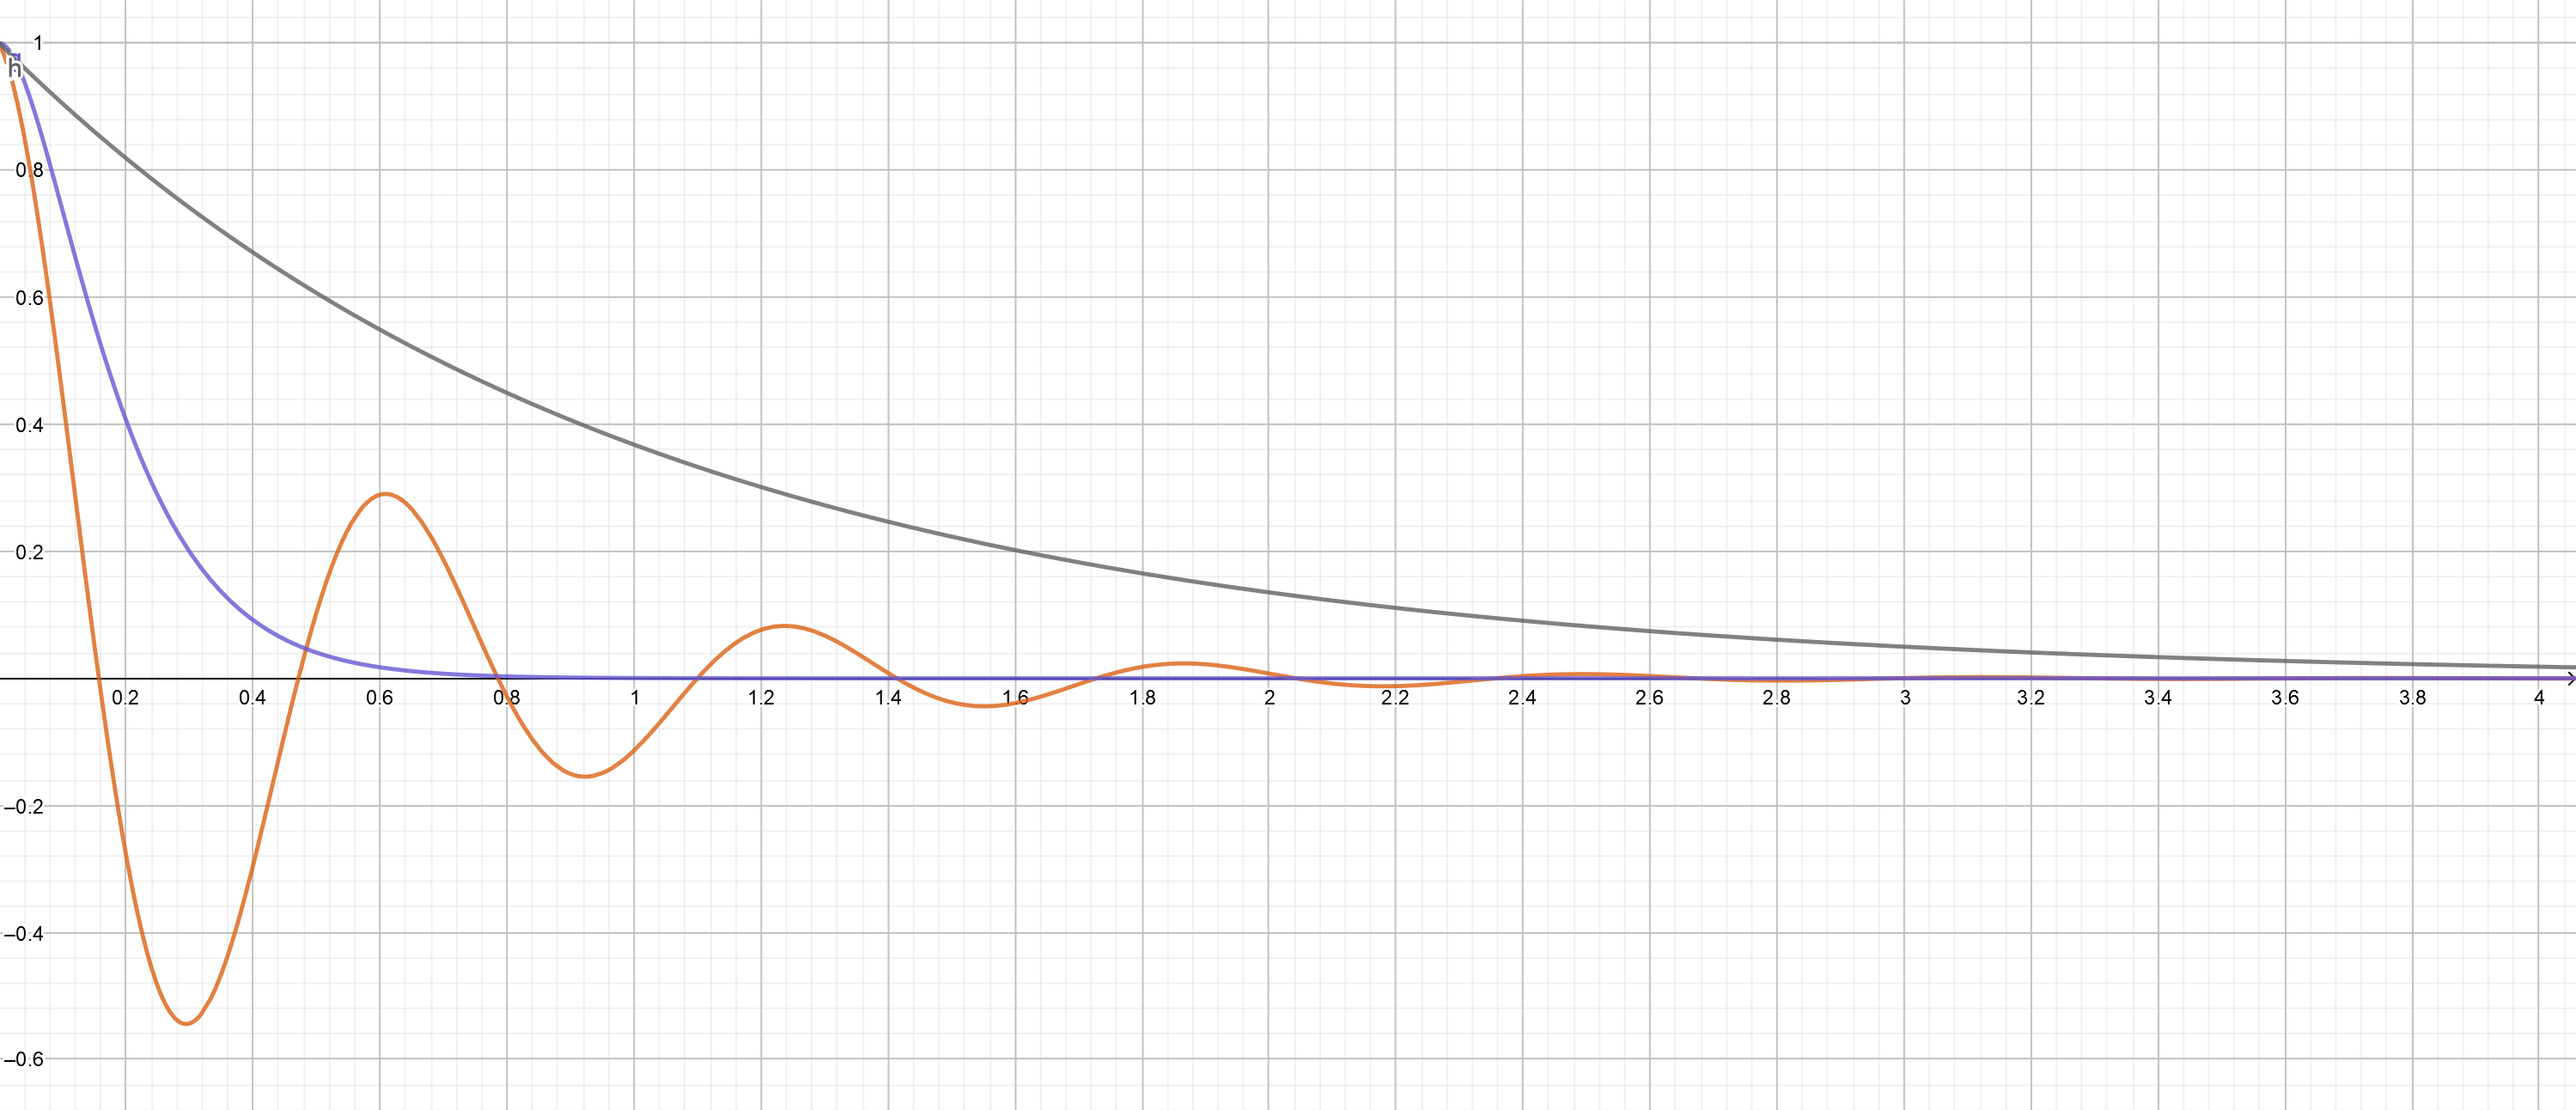
\includegraphics[width=.9\textwidth]{Preparation/damping_cases.png}
        \caption[Damping cases of a harmonic oscillation]{Plot of amplitude against time of a harmonic oscillation with
        parameterized damping coefficient. Orange: underdamped, Gray: overdamped, Blue: critically damped.}
        \label{fig:damping_cases_prepTask_2}
    \end{figure}
    %
    \subsection{Unknown Angular Inertia of the Pendulum}\label{sec:preparation_task_3}
    %
        The angular inertia of the pendulum \( J_P \) can be determined by adding a known angular inertia \( J_R \) of a cylindrical rod. As \cref{eq:DEParameters} delivers
        %
        \begin{equation}
            \omega_0=\sqrt{\frac{D^*}{J}}
        \end{equation}
        %
        and \( \omega=\frac{2\pi}{T} \), the following relation is given:
        %
        \begin{align}
            \omega_{0,P}=\sqrt{\frac{D^*}{J_P}}=\frac{2\pi}{T_P} \quad              &\Leftrightarrow \quad 2\pi=T_P\cdot\sqrt{\frac{D^*}{J_P}} \label{eq:omegaP} \\
            \omega_{0,P+R}=\sqrt{\frac{D^*}{J_P+J_R}}=\frac{2\pi}{T_{P+R}} \quad    &\Leftrightarrow \quad 2\pi=T_{P+R}\cdot\sqrt{\frac{D^*}{J_P+J_R}} \label{eq:omegaP+R}
        \end{align}
        %
        When \cref{eq:omegaP} and \cref{eq:omegaP+R} are equated:
        %
        \begin{align}
                                    &T_P\cdot\sqrt{\frac{D^*}{J_P}}=T_{P+R}\cdot\sqrt{\frac{D^*}{J_P+J_R}} \nonumber\\
            \Leftrightarrow \quad   &\left( \frac{T_{P+R}}{T_P} \right)^2 =\frac{J_P+J_R}{J_P}=1+\frac{J_R}{J_P} \nonumber\\
            \Leftrightarrow \quad   &\frac{J_R}{J_P}=\left( \frac{T_{P+R}}{T_P} \right)^2-1 \nonumber\\
            \Rightarrow \quad       &J_P=\frac{J_R}{\left( \frac{T_{P+R}}{T_P} \right)^2-1}
            \label{eq:inertia}
        \end{align}
        %
        The angular inertia of the pendulum can be calculated without knowing the torsion constant \( D^* \).
        %
    \subsection{Rotational Inertia of a Cylindrical Rod}\label{sec:preparation_task_4}
        %
        \begin{figure}[h]
            \centering
            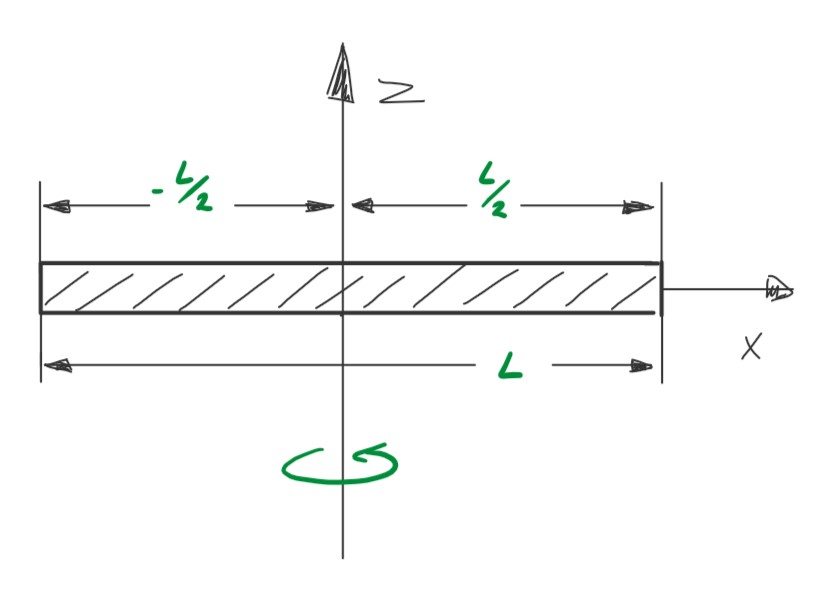
\includegraphics[width=.6\textwidth]{Preparation/rotating_rod.jpg}
            \caption[Rotating rod]{Scheme of an orthogonally to its center axis rotating rod.}
            \label{fig:rotationalIntertia_of_Cyl}
        \end{figure}
        %
        Inertia of a rotating mass dimensionless mass is proportional to the square of the distance to its rotational axis.
        As the mass of a cylindrical body is distributed over its volume, it is necessary to integrate over all \( dm  \) along
        the distance \( r \) from the center of rotation. \cite{Eichler.2016}
        \begin{equation}
            J_Z = \int r^2 dm
            \label{eq:rotationalIntertia_of_Cyl}
        \end{equation}
        With
        \begin{equation}
            \rho = \frac{dm}{dx} = \frac{M}{L} \qquad \Leftrightarrow \qquad dm = \frac{M}{L} dx
        \end{equation}
        plugged into \cref{eq:rotationalIntertia_of_Cyl} with respect to the integration limits as of \cref{fig:rotationalIntertia_of_Cyl}
        gives
        \begin{equation}
            J_Z = \int_{-\nicefrac{L}{2}}^{\nicefrac{L}{2}} \frac{M}{L} x^2 dx = \frac{1}{12}M L^2
            \label{eq:rotationalIntertia_of_Cyl alternate}
        \end{equation}
        %
    \subsection{Equations for the Sensor Capacitances}\label{sec:preparation_task_5}
        To derive:
        \begin{align}
            C_1(\varphi) = \varepsilon_0 \frac{\pi D^2}{16 d} \left( 1 - \frac{2\varphi}{\pi} \right) \\
            C_2(\varphi) = \varepsilon_0 \frac{\pi D^2}{16 d} \left( 1 + \frac{2\varphi}{\pi} \right)
        \end{align}
        with
        \begin{equation}
            A_{1,2}(\varphi) = \frac{1}{16}\pi D^2 \left( 1 \pm \frac{2\varphi}{\pi} \right)
        \end{equation}
        %
        \begin{figure}[h]
            \centering
            \subfloat[Rotor at \( \varphi = 0 \)\label{subfig:rotorAt.5pi}]{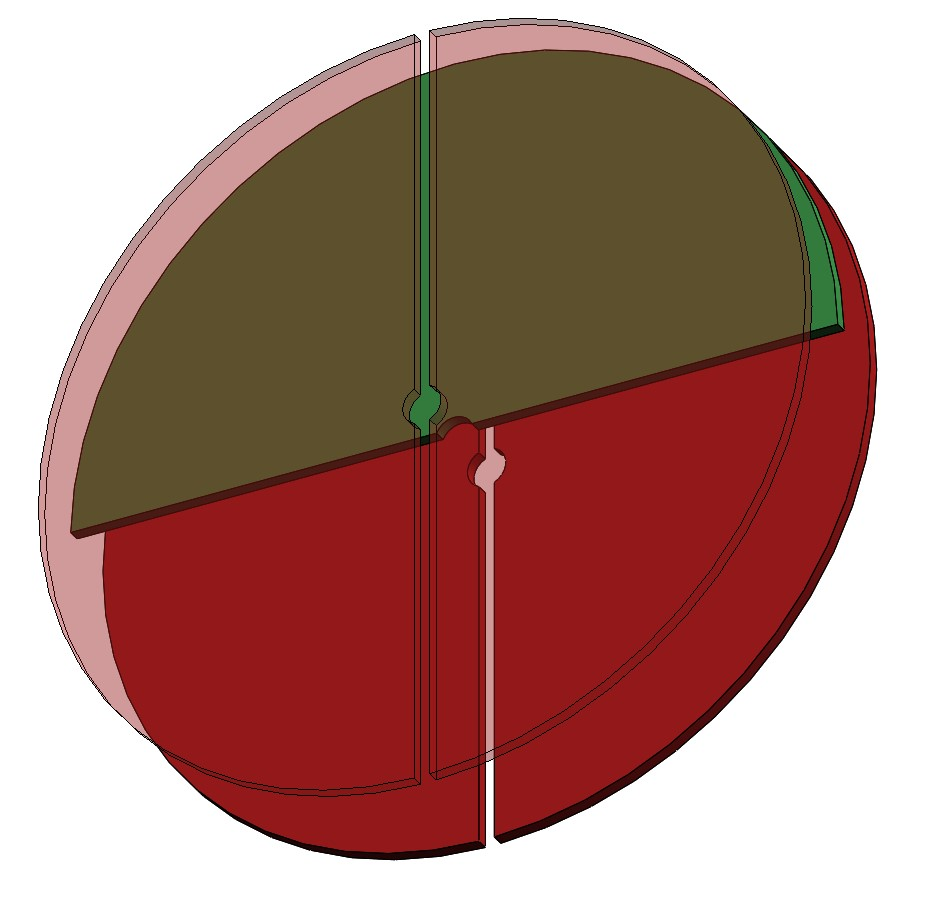
\includegraphics[width=.3\textwidth]{aufbau/statorRotorStator_0.5pi.jpg}}
            \subfloat[Rotor at \( \varphi = \pm \frac{\pi}{2} \)\label{subfig:rotorAtpi}]{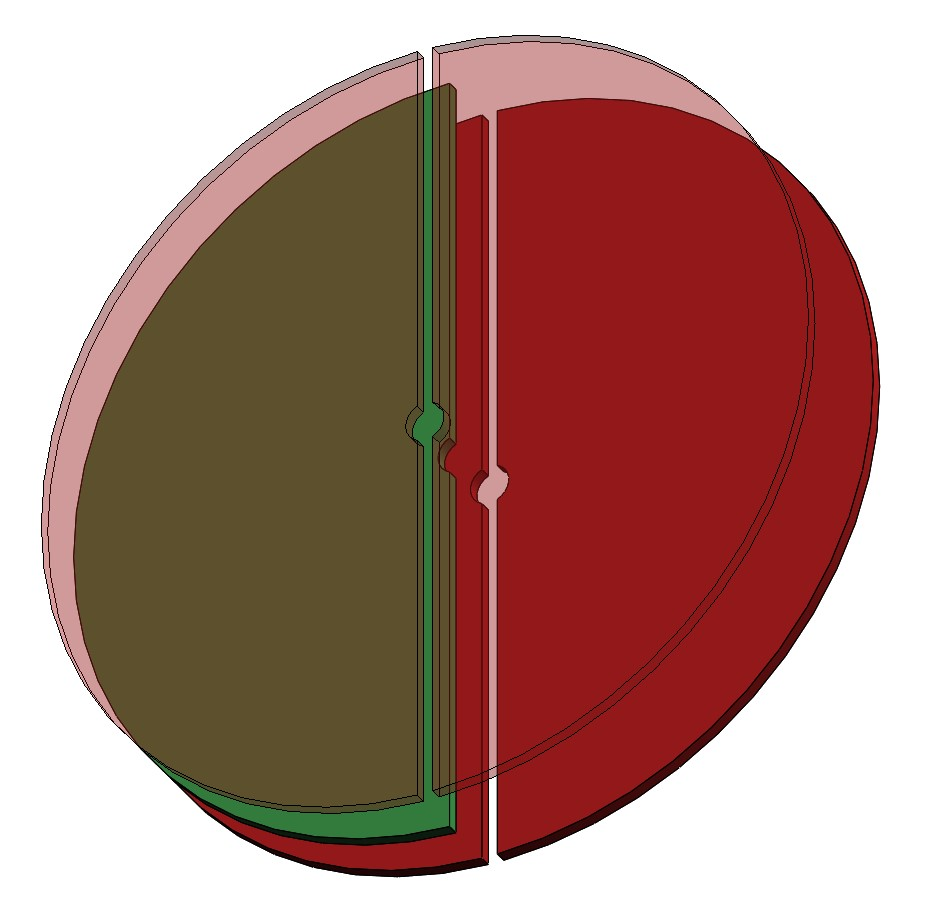
\includegraphics[width=.3\textwidth]{aufbau/statorRotorStator_pi.jpg}}
            \subfloat[Rotor at \( \varphi = \mp \frac{\pi}{2} \)\label{subfig:rotorAt0}]{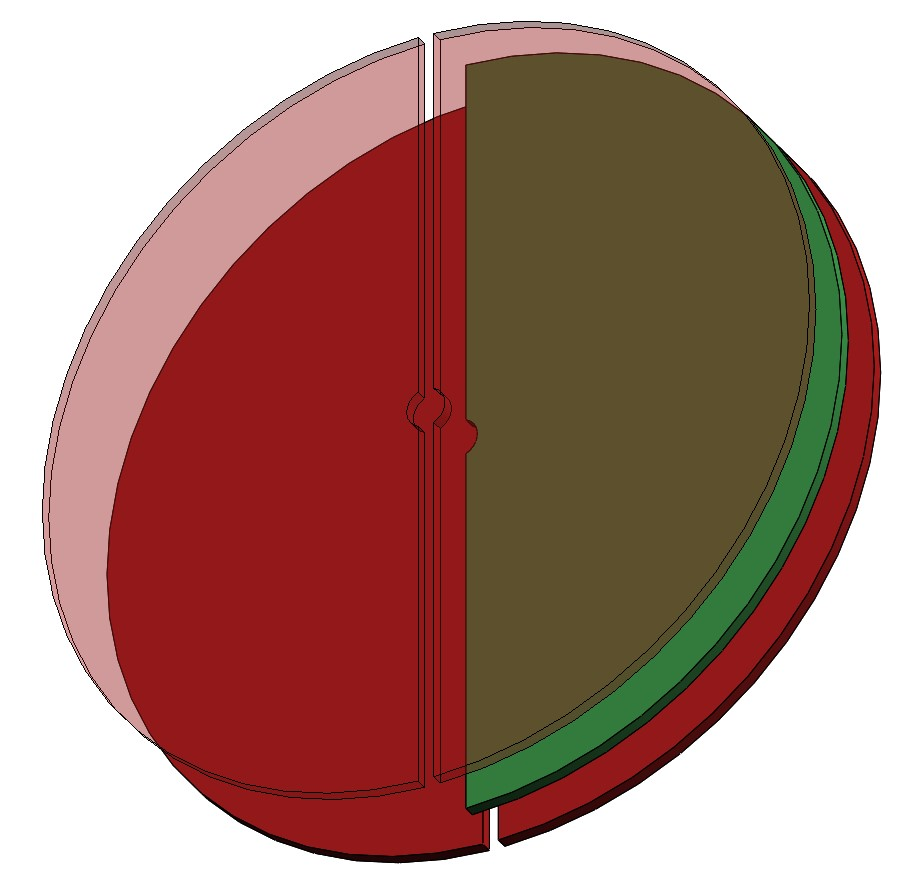
\includegraphics[width=.3\textwidth]{aufbau/statorRotorStator_0.jpg}}
            \caption[Schematical assembly of the angular sensor]{Schematical assembly of the angular sensor. The semi circular rotor plate (green) sandwiched between the two stators (red). The area of the rotor facing one of the vertical stator
            pairs varies with the angular displacement \( \varphi \)
            of the rotor.}
            \label{fig:rotorPositions}
        \end{figure}
        %
        One half of the stator pairs together with the rotor plate forms two capacitors connected in series. With each
        capacitor having the same value at any time the total capacitance equates to
        \begin{equation}
            C_{1,2}(\varphi) = \varepsilon_0 \varepsilon_r \frac{A(\pm\varphi)}{2d}
            \label{eq:angularCapacitance}
        \end{equation}
        Where \( A(\varphi) \) can be expressed as
        \begin{align}
            A(\varphi) = \frac{1}{8}D^2 \left( \pi \pm \varphi \right) \nonumber \\
            A(\varphi) = \frac{1}{8}D^2 \left( \frac{\pi^2}{\pi} \pm \frac{\pi\varphi}{\pi} \right) \nonumber \\
            A(\varphi) = \frac{1}{8} \pi D^2 \left( 1 \pm \frac{\varphi}{\pi}\right)
            \label{eq:angularDependencyOfTheArea}
        \end{align}
        Say the zero position is chosen such as the whole area of the rotor takes effect (see \cref{subfig:rotorAt0})
        \cref{eq:angularDependencyOfTheArea} maximizes. Thus, the absolute capacitance of one of the capacitors is maximized.
        Stepping the rotor about \( \varphi = \frac{\pi}{2} \) as seen in \cref{subfig:rotorAt.5pi} halves the
        effective area of the capacitor halving the total capacitance. At an angular displacement of \( \varphi = \pi \)
        the capacitance equates to zero respectively.\\
        Combining \cref{eq:angularCapacitance} and \cref{eq:angularDependencyOfTheArea} gives \footnote{The solution is missing a factor of 2 in front of \(\varphi\)}
        \begin{equation}
            C_{1,2} = \varepsilon_0 \frac{\pi D^2}{16d} \left( 1 \pm \frac{2\varphi}{\pi} \right)
        \end{equation}
        %
        \begin{equation}
            \left(1 \pm \frac{2\varphi}{\pi} \right)
            \begin{cases}
                = 0 \quad \text{for} \quad \varphi = \pm \frac{\pi}{2} \nonumber \\
                = 1 \quad \text{for} \quad \varphi = 0 \nonumber \\
                = 2 \quad \text{for} \quad \varphi = \mp \frac{\pi}{2} \nonumber
            \end{cases}
        \end{equation}
        %
    \subsection{Time to Reach the Threshold Voltage}\label{sec:preparation_task_6}
        %
        The charging curve of a capacitor is given by \cref{eq:chargingCurve}.
        \begin{equation}
            U_C(t) = U_0 ( 1-e^{-\frac{t}{\tau}})
            \label{eq:chargingCurve}
        \end{equation}
        Being interested at the time \( t_{th} \) it takes to reach a certain threshold voltage \( U_{th} \), \cref{eq:chargingCurve}
        can be transformed as follows:
        \begin{gather}
            1- \frac{U_{th}}{U_0} = e^{-\frac{t_{th}}{\tau}} \nonumber \\
            \Leftrightarrow \nonumber \\
            t_{th} = - \ln\left(1- \frac{U_{th}}{U_0}\right) \cdot \tau
            \label{eq:timeToThresholfVoltage}
        \end{gather}
        with the time constant \( \tau = R \cdot C \).
        %
    \subsection{Determining the Angular Deflection by the Difference of Timer Ticks}\label{sec:preparation_task_7}
        %
        The time to reach the threshold voltage as of \cref{eq:timeToThresholfVoltage} is captured independently due to
        each capacitor being connected to individual GPIOs.\par
        Since the charging curve of the capacitors differs in an anti-proportional manner when an angular deflection takes
        place the absolute value of the time difference gives the angle about zero while the sign gives the direction.
        Therefore, taken these considerations in account and merging \cref{eq:angularCapacitance} and \cref{eq:timeToThresholfVoltage}
        gives:
        \begin{align}
            \Delta t_{th}(\varphi)   &= t_{th,1} - t_{th,2} = -\ln\left( 1- \frac{U_{th}}{U_0} \right)R\left[ C_1(\varphi) - C_2(\varphi) \right] \nonumber \\
                            &= -\varepsilon_0 R \frac{\pi D^2}{16d} \ln\left( 1 - \frac{U_{th}}{U_0} \right) \left[ \left( 1 + \frac{2\varphi}{\pi} \right) - \left( 1 - \frac{2\varphi}{\pi} \right) \right] \nonumber \\
                            &= -\varepsilon_0 R \frac{4D^2}{16d} \ln\left( 1 - \frac{U_{th}}{U_0} \right) \cdot \varphi
            \label{eq:time_to_reach_thresholdVoltage}
        \end{align}
        Here \( \varepsilon_0 \), \( R \), \( D \), \( d \), \( U_{th} \) and \( U_0 \) remain constant and can be gathered as a proportionality
        factor. This reduces \cref{eq:time_to_reach_thresholdVoltage} to
        \begin{equation}
            \Delta t_{th}(\varphi) = \chi \cdot \varphi
            \label{eq:simplified_time_to_reach_thresholdVoltage}
        \end{equation}
        The \micro C checks the state of the input pin once every cycle. To take that into account the difference in threshold time
        \( \Delta t_{th} \) has to be divided by the cycle time \( \Delta t \) of the \micro C which gives the number of cycles it took for the
        input pins to switch state from low to high. If a change takes place at a non integer multiple of \( \Delta t \)
        the \micro C will register a transition on the subsequent cycle, thus, for the cycle count \( n \) applies \( n \in \mathbb{N} \).
        Furthermore, a non-integer value for \( n \) has to be rounded up to the next integer value.

        Mathematically the above considerations yield
        \begin{equation}
            n(\varphi) = \left\lceil \frac{\left\vert \Delta t_{th}(\varphi) \right\vert }{\Delta t} \right\rceil = \left\lceil \chi' \cdot \vert\varphi\vert \right\rceil \qquad \text{with} \qquad n(\varphi): n(\varphi) \in \mathbb{N}
            \label{eq:value_of_cycle_Count}
        \end{equation}
        which translates into the amount of deflection and
        \begin{equation}
            \frac{\vert n(\varphi)\vert}{n(\varphi)} = \pm 1
            \label{eq:sign_of_cycle_count}
        \end{equation}
        to distinguish between a CW/CCW rotation.
        %
    \subsection{Sensitivity of the Angular Sensor}\label{sec:preparation_task_8}
        %
        As seen in \cref{eq:simplified_time_to_reach_thresholdVoltage} the tick rate relates linearly with the angular displacement \( \varphi \).
        Therefore, the maximum resolution of the angular sensor expressed as \textit{ticks per radiant} \textbf{is} \( \chi' \).
        \begin{equation}
            \frac{dn(\varphi)}{d\varphi} = \chi' \cdot \varphi \frac{d}{d\varphi} = \chi'
        \end{equation}
        \begin{figure}[H]
            \centering
            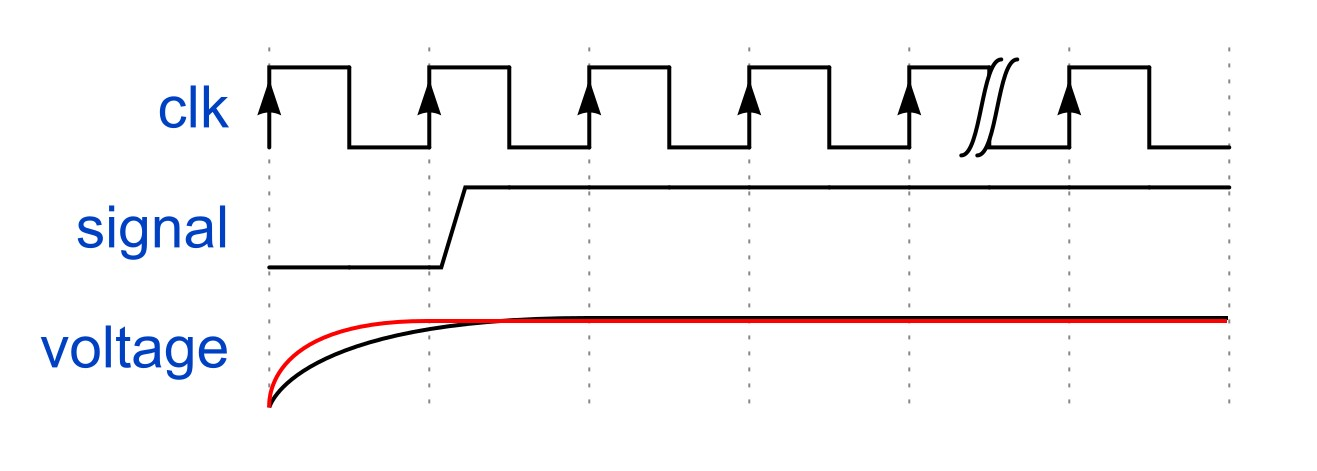
\includegraphics[width=.7\textwidth]{aufbau/clk_signal_timing_diagram.jpg}
            \caption[Timing diagram showing the signal transition]{Timing diagram showing the signal transition.}
            \label{fig:timing_diagram}
        \end{figure}
        The clock frequency of the \micro C is \( f = \SI[]{16}[]{MHz} \) which gives a cycle time of \( \delta t = \SI[]{62.5}[]{ns} \).
        
        To ready the capacitors for the next charging cycle they need to be discharged as quick as possible. Considering
        that a time to discharge the capacitors \( < \Delta t \) makes no significant difference the unknown value \( R \)
        of the resistor can be approximated as
        \begin{gather}
            3\tau = \Delta t = 3RC \nonumber \\
            \Leftrightarrow \nonumber \\
            \frac{\Delta t}{3C_{max}} = R
            \label{eq:resistor_approximation}
        \end{gather}
        In the equation above the assumptions are made that a discharge rate of 95\% is sufficient and the circuit needs
        to be able to discharge the capacitor within the timeframe \( \Delta t \) while being at its maximum capacitance.
        Thus,
        \begin{align}
            C_{max} &= \varepsilon_0 \frac{\pi D^2}{8d} \nonumber \\
                    &= \SI{8,85\cdot10^{-12}}{\frac{\ampere\second}{\volt\metre}} \frac{\pi \cdot \SI{0.12^2}{m^2}}{8 \cdot \SI{0.01}{m}} \nonumber \\
                    &= \SI{5.01}{pF}
            \label{val:C_max}
        \end{align}
        in \cref{eq:resistor_approximation} gives a value for the resistance as
        \begin{equation}
            \frac{\SI{62.5}{ns}}{3 \cdot \SI{5.01}{pF}} \approx \SI{4160.9}{k\ohm}
        \end{equation}
        This lies between the two more common E-Series values of \SI{4.7}{k\ohm} and \SI{3.9}{k\ohm}. For further calculations
        the latter is chosen as a higher resistance would increase the discharge time.\par\medskip
        Plugging in the given values of for \( \varepsilon_0, D, d, U_{th}, U_0 \) and the calculated values for \( \Delta t \text{ and } R \)
        equates \cref{eq:simplified_time_to_reach_thresholdVoltage} to
    
        \begin{align}
            \chi'   &= -\varepsilon_0 R \frac{4 D^2}{16d} \ln\left( 1 - \frac{U_{th}}{U_0} \right) \Delta t^{-1} \nonumber \\
                    &= -\SI{8.85 \cdot 10^{-12}}{\frac{As}{Vm}} \cdot \SI{3.9}{k\ohm} \cdot \frac{4 \cdot \SI{0.12^2}{\metre\squared}}{16 \cdot \SI{0.01}{\metre}} \ln\left( 1 - \frac{\SI{2.5}{\volt}}{\SI{5}{\volt}} \right) \cdot \frac{1}{\SI{62.5}{ns}} \nonumber \\
                    &\approx \SI{0.138}{\radian^{-1}}
        \end{align}
\chapter{Set-Up of Experiment}
%
	The equipment and materials that are needed to perform the experiments are shown in \cref{fig:setup_total}. A detailed
	view of the angular sensor assembly is seen in \cref{fig:setup_detailed}.\par
	Using a desktop computer a serial connection via USB to the \micro C board is established. A serial monitor - \textsc{RealTerm} - is used to
	log the inbound stream send by the \micro C. The relevant settings are listed below:\par
	\begin{itemize}
		\item \SI{9600}{Baud}
		\item On the \texttt{Display} tab, \texttt{Ascii} and \texttt{new Line mode} are checked, \texttt{Direct capture}
		remains un-checked.
		\item COM-Port as assigned by the OS.
	\end{itemize}
	%
	The data is now continuously sent by the \micro C. The data is displayed on the screen. A text file is created in
	which the data is written and saved. Two columns are displayed. The first column contains the time $t$ in seconds, the
	second the number of timer ticks $n$. The current source for the electromagnet is switched on.\par
	Now the setup is completed and the experiments can be started.
	%
	\begin{figure}[h]
		\centering
		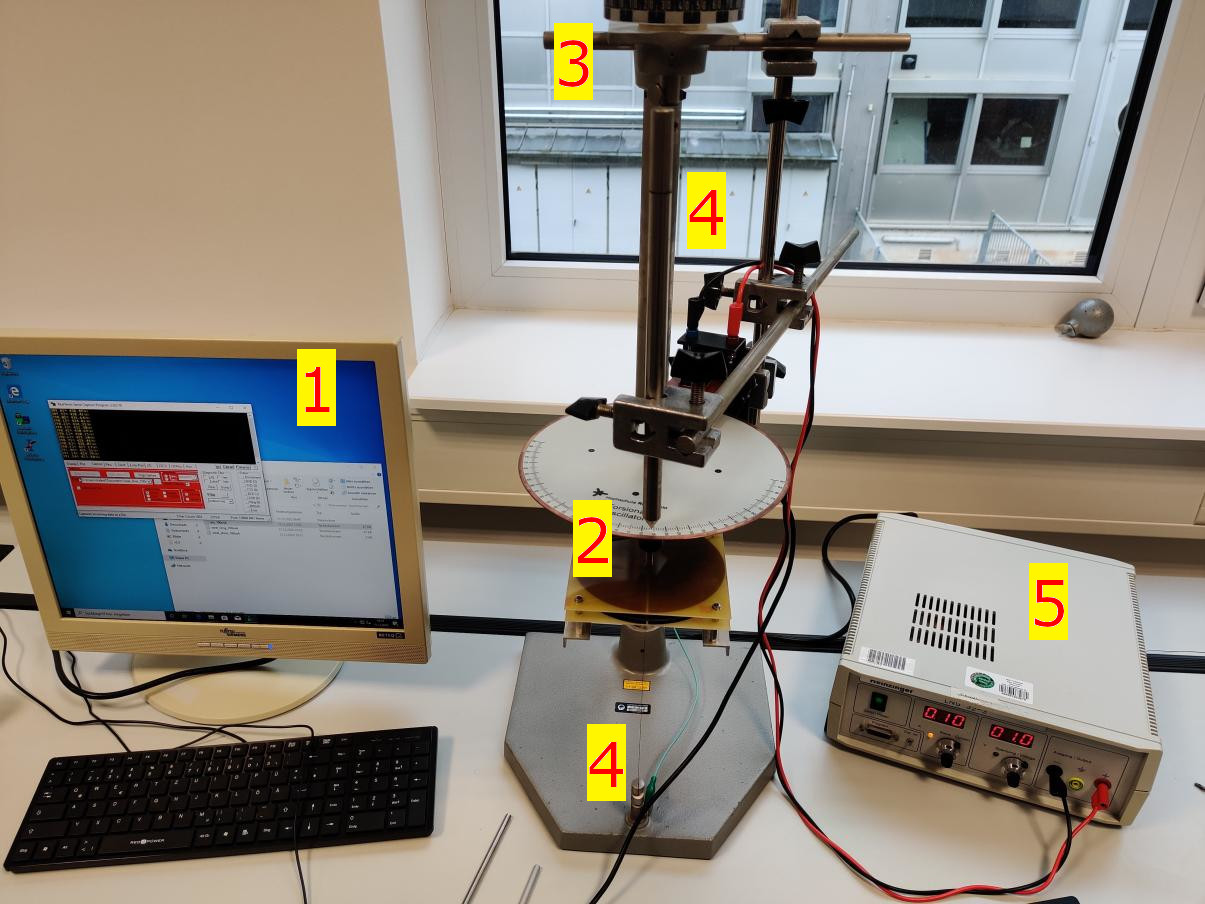
\includegraphics[width=.8\textwidth]{aufbau/setup_total_num.jpg}
		\caption[Equipment used.]{ Equipment and material required for the experiments. 1. Computer running \textsc{RealTerm}, 2. Angular sensor assembly,
		3. Zero adjustment, 4. Torsion wire, 5. PSU in constant current mode powering the eddy current brake.}
		\label{fig:setup_total}
	\end{figure}
	%
	\par
	%
	\begin{figure}[h]
		\centering
		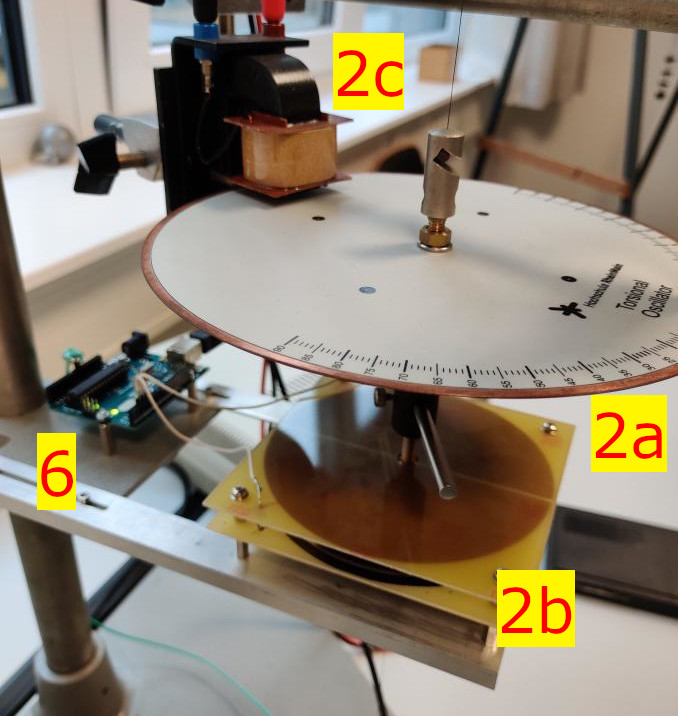
\includegraphics[width=.5\textwidth]{aufbau/setup_pendulum_side_num.jpg}
		\caption[Equipment in detail.]{ Detailed view of the angular sensor assembly. 2a: Copper plate with scale in degree, 2b: Capacitor plates, 2c: Eddy current brake,
		6: \micro C board.}
		\label{fig:setup_detailed}
	\end{figure}
	%
\input{chapters/4_durchführung}
\chapter{Evaluation}
    \section{Angular Sensor}
        Before investigating the dependence of the angle and the timer ticks, it is needed to determine the mean value of the timer
        ticks for each angle. The mean values are computed taking 20 samples each.\par
        \begin{table}[h]
            \caption[Mean value of timer ticks per angular displacement]{Mean value of timer ticks per angular displacement}
            \centering
            \begin{tabular}{@{}S[table-format=+2]S[table-format=3.2]cS[table-format=+2]S[table-format=+3.2]@{}}
                \toprule
                \varphi / \si[]{\degree}            &\bar{n}        &\hspace{20mm}  &\varphi / \si[]{\degree}   &\bar{n}\\
                \midrule
                +90                                 &601.34         &               &-10                        &-55.33\\
                +80                                 &549.63         &               &-20                        &-126.04\\
                +70                                 &482.26         &               &-30                        &-195.80\\
                +60                                 &421.93         &               &-40                        &-262.31\\
                +50                                 &353.10         &               &-50                        &-331.20\\
                +40                                 &288.13         &               &-60                        &-396.87\\
                +30                                 &220.58         &               &-70                        &-459.46\\
                +20                                 &147.85         &               &-80                        &-474.44\\
                +10                                 &83.57          &               &-90                        &-499.79\\
                +0                                  &14.36          &               &                           &\\
                \bottomrule
            \end{tabular}
            \label{tab:mean ticks per angle}
        \end{table}
        %
        In \cref{fig:angular-sensor} the timer ticks \(n\) are plotted as a function of the angle \(\varphi\).
        %
        \begin{figure}[H]
            \centering
            \includegraphics[width=1\linewidth]{"messdaten/Angular Sensor"}
            \caption[Curve of the angular sensor]{Curve of the angular sensor}
            \label{fig:angular-sensor}
        \end{figure}
        %
        The sensitivity corresponds to the slope of the curve and the offset to the intercept.\par
        The computed fit is
        %
        \begin{equation}
            n(\varphi)=\SI{373.60}{rad^{-1}}\cdot\varphi +19.03
        \end{equation}
        %
        which gives values for the sensitivity \( s \) and the offset \( o \) of
        %
        \begin{align}
            s&=\SI{374}{rad^{-1}} \pm \SI{1}{rad^{-1}}\\
            o&=19 \pm 1
        \end{align}\par\medskip
        %
        In comparison with the estimated sensitivity of \(\SI{0.138}{rad^{-1}}\)(\cref{eq:est.sensitivity}) is off by
        an order of 4. Provided the captured data is accurate it appears reasonable to discard the estimates.\par
    \section{Torsional Pendulum}
    %
        \subsection{Natural Angular Frequency and Damping Coefficient}
            \Cref{fig:damped-oscillation-100mA} shows the oscillation with a coil current of \(\SI{100}{mA}\). The respective plots
            for coil currents ranging from \(\SI{200-500}{mA}\) and the coil current turned off can be seen in \cref{fig:damped-oscillations}.
            Deflection is plotted versus time. The period time for each curve is determined by reading a few values and building the mean.\par
            %
            \begin{figure}[H]%
                \centering
                \includegraphics[width=1\linewidth]{"messdaten/Damped Oscillation (100mA)"}
                \caption[Course of the tick rate at \(I_{c}=\SI{100}{mA}\)]{Plot of the tick rate over time with a coil current of \SI{100}{mA}.}
                \label{fig:damped-oscillation-100mA}
            \end{figure}
            %
            The values are as follows:\par
            \begin{table}[h]
                \centering
                \caption[Period times for the damped oscillations]{}
                \begin{tabular}{@{}llll@{}}
                    \toprule
                    \( T_0 \)       &$\SI{9.7}{s} \pm \SI{0.5}{s}$    &\hspace{10mm}\(T_{300}\)      &$\SI{9.8}{s} \pm \SI{0.5}{s}$\\
                    \( T_{100} \)   &$\SI{9.6}{s} \pm \SI{0.5}{s}$    &\hspace{10mm}\(T_{400}\)      &$\SI{10.0}{s} \pm \SI{0.5}{s}$\\
                    \(T_{200}\)     &$\SI{9.6}{s} \pm \SI{0.5}{s}$    &\hspace{10mm}\(T_{500}\)      &$\SI{10.4}{s} \pm \SI{0.5}{s}$\\
                    \bottomrule
                \end{tabular}
                \label{tab:period_times_damped_oscillations}
            \end{table}
            %
            Thus, the damped natural frequencies are calculated using \(\omega=\frac{2\pi}{T}\):\par
            \begin{table}[h]
                \centering
                \caption[Damped natural frequencies]{}
                \begin{tabular}{@{}llll@{}}
                    \toprule
                    $\omega_{d,0}$      &$\SI{0.65}{s^{-1}} \pm \SI{0.03}{s^{-1}}$  &\hspace{10mm}$\omega_{d,300}$  &$\SI{0.64}{s^{-1}} \pm \SI{0.03}{s^{-1}}$\\
                    $\omega_{d,100}$    &$\SI{0.65}{s^{-1}} \pm \SI{0.03}{s^{-1}}$  &\hspace{10mm}$\omega_{d,400}$  &$\SI{0.63}{s^{-1}} \pm \SI{0.03}{s^{-1}}$\\
                    $\omega_{d,200}$    &$\SI{0.64}{s^{-1}} \pm \SI{0.03}{s^{-1}}$  &\hspace{10mm}$\omega_{d,500}$  &$\SI{0.60}{s^{-1}} \pm \SI{0.03}{s^{-1}}$\\
                    \bottomrule
                \end{tabular}
                \label{tab:damped_natural_frequencies}
            \end{table}
            %
            The deviations of the period time are reading errors. The ones of the damped natural frequency can be calculated with\par
            %
            \begin{align}
                \Delta \omega_d &=\left|\frac{\partial \omega_d}{\partial T}\right| \cdot \Delta T \nonumber \\
                                &=\frac{2\pi}{T^2}\cdot \Delta T
            \end{align}
            %
            for \(\omega_{d,0}\) e.g.:\par
            %
            \begin{align}
                \Delta\omega_{d,0}  &=\frac{2\pi}{(\SI{9.7}{s})^2}\cdot \SI{0.5}{s} \nonumber \\
                                    &=\SI{0.03}{s^{-1}}
            \end{align}
            %
            The damping coefficient can be determined by way of\par
            %
            \begin{align}
                \varphi_1 \cdot e^{-\delta t_0} &=\varphi_0 \cdot e^{-\delta t_1} \nonumber \\%   &&\Bigg|\cdot \frac{e^{\delta t_1}}{\varphi_1} \nonumber\\
                e^{\delta(t_1-t_0)}             &=\frac{\varphi_0}{\varphi_1} \nonumber \\%       &&\Bigg|\ln \nonumber\\
                \delta(t_1-t_0)                 &=\ln{\frac{\varphi_0}{\varphi_1}} \nonumber \\%  &&\Bigg|\cdot \frac{1}{(t_1-t_0)} \nonumber\\
                \delta                          &=(t_1-t_0)^{-1}\cdot\ln{\frac{\varphi_0}{\varphi_1}}
            \end{align}
            %
            The times and angles have been read and \(\delta\) has been calculated individually.\par
            This gives us the following mean values:\par
            %
            \begin{table}[h]
                \centering
                \caption[Mean values of the dampening coefficient]{}
                \begin{tabular}{@{}llll@{}}
                    \toprule
                    $\delta_0$        &$\SI{0.002}{s^{-1}} \pm \SI{0.001}{s^{-1}}$  &\hspace{10mm}$\delta_{300}$ &$\SI{0.08}{s^{-1}} \pm \SI{0.01}{s^{-1}}$\\
                    $\delta_{100}$    &$\SI{0.008}{s^{-1}} \pm \SI{0.002}{s^{-1}}$  &\hspace{10mm}$\delta_{400}$ &$\SI{0.12}{s^{-1}} \pm \SI{0.01}{s^{-1}}$\\
                    $\delta_{200}$    &$\SI{0.03}{s^{-1}} \pm \SI{0.01}{s^{-1}}$    &\hspace{10mm}$\delta_{500}$ &$\SI{0.22}{s^{-1}} \pm \SI{0.01}{s^{-1}}$\\
                    \bottomrule
                \end{tabular}
                \label{tab:dampening_coefficients}
            \end{table}
            %
            For the deviation, the standard deviation is used. Otherwise, it can also be determined by means of the partial derivation:\par
            %
            \begin{align}
                \Delta\delta    &= \left| \frac{\partial\delta}{\partial t_1} \right| \cdot \Delta t_1 + \left| \frac{\partial\delta}{\partial t_0} \right| \cdot \Delta t_0 + \left| \frac{\partial\delta}{\partial \varphi_0} \right| \cdot \Delta \varphi_0 + \left| \frac{\partial\delta}{\partial \varphi_1} \right| \cdot \Delta \varphi_1 \nonumber\\
                                &= \frac{1}{(t_1-t_0)^2} \cdot \ln{\frac{\varphi_0}{\varphi_1}} \cdot (\Delta t_0 + \Delta t_1) + \frac{1}{(t_1-t_0)} \cdot \left( \frac{1}{\varphi_0} \cdot \Delta\varphi_0 + \frac{1}{\varphi_1} \cdot \Delta\varphi_1 \right)
            \end{align}%
            The natural angular frequencies are calculated via $ \omega_0=\sqrt{\omega_d^2+\delta^2} $ as\par
            %
            \begin{table}[h]
                \centering
                \caption[Angular natural frequencies]{}
                \begin{tabular}{@{}llll@{}}
                    \toprule
                    $\omega_{0,0}$      &$\SI{0.65}{s^{-1}} \pm \SI{0.03}{s^{-1}}$  &\hspace{10mm}$\omega_{0,300}$   &$\SI{0.65}{s^{-1}} \pm \SI{0.03}{s^{-1}}$\\
                    $\omega_{0,100}$    &$\SI{0.65}{s^{-1}} \pm \SI{0.03}{s^{-1}}$  &\hspace{10mm}$\omega_{0,400}$   &$\SI{0.64}{s^{-1}} \pm \SI{0.03}{s^{-1}}$\\
                    $\omega_{0,200}$    &$\SI{0.64}{s^{-1}} \pm \SI{0.03}{s^{-1}}$  &\hspace{10mm}$\omega_{0,500}$   &$\SI{0.68}{s^{-1}} \pm \SI{0.03}{s^{-1}}$\\
                    \bottomrule
                \end{tabular}
                \label{tab:angular_natural_frequencies}
            \end{table}
            %
            and their deviations via\par
            %
            \begin{align}
                \Delta\omega_0  &=\left| \frac{\partial\omega_0}{\partial\omega_d} \right| \cdot \Delta\omega_0 + \left| \frac{\partial\omega_0}{\partial\delta} \right| \cdot \Delta\delta \nonumber\\
                                &=\frac{\omega_d}{\sqrt{\omega_d^2+\delta^2}} \cdot \Delta\omega_d + \frac{\delta}{\sqrt{\omega_d^2+\delta^2}} \cdot \Delta\delta
            \end{align}
            %
            for \(\omega_{0,0}\) e.g. as\par
            %
            \begin{align*}
                \Delta\omega_{0,0}  &=\frac{\SI{0.65}{s^{-1}}}{\sqrt{\SI{0.65}{s^{-1}}+\SI{0.002}{s^{-1}}}} \cdot \SI{0.03}{s^{-1}} + \frac{\SI{0.002}{s^{-1}}}{\sqrt{\SI{0.65}{s^{-1}}+\SI{0.002}{s^{-1}}}} \cdot \SI{0.001}{s^{-1}}\\
                                    &=\SI{0.03}{s^{-1}}+\SI{3}{\cdot10^{-6}s^{-1}}\\
                                    &\approx\SI{0.03}{s^{-1}}
            \end{align*}
            %
            In \cref{fig:damping-coefficient} the damping coefficient is plotted versus coil current. For finding a formula
            \(\delta(I)\) SciDAVis did an exponential fit \(\delta_e(I)\) (red curve) and a fourth degree polynomial fit
            \(\delta_p(I)\) (blue curve):\par
            %
            \begin{align}
                \delta_e(I)=&\SI{0.013}{s^{-1}}\cdot e^{\SI{0.0052}{A^{-1}}\cdot I}\\
                \delta_p(I)=&\SI{1.8}{\cdot 10^{-3}s^{-1}} - \SI{1.5}{\cdot 10^{-5}s^{-1}A^{-1}}\cdot I + \SI{6.4}{\cdot 10^{-7}s^{-1}A^{-2}}\cdot I^2 \nonumber\\
                            &+ \SI{1.2}{\cdot 10^{-9}s^{-1}A^{-3}}\cdot I^3 + \SI{2.2}{\cdot 10^{-12}s^{-1}A^{-4}}\cdot I^4
            \end{align}
            %
            \begin{figure}
                \centering
                \includegraphics[width=1\linewidth]{"messdaten/Damping Coefficient"}
                \caption[Damping coefficient depending on the coil current]{Damping coefficient depending on the coil current}
                \label{fig:damping-coefficient}
            \end{figure}
            %
            As it can be seen, the polynomial fit is a better approximation than the exponential. However, the polynomial curve
            is only a good approach in the area of \(0 \leq I \leq \SI{500}{mA}\). At higher currents the curve has a maximum
            and goes lower again, which is illogical in the physical sense. Therefore, the exponential curve is a qualitatively
            better description of the dependency.\par\medskip
            Finally, the aperiodic case is considered and plotted in \cref{fig:damped-oscillation-aperiodic}.\par
            %
            \begin{figure}
                \centering
                \includegraphics[width=1\linewidth]{"messdaten/Damped Oscillation (aperiodic)"}
                \caption[Aperiodic damped oscillation at \(I_c=\SI{1.3}{A}\)]{Aperiodic damped oscillation at \(I_c=\SI{1.3}{A}\)}
                \label{fig:damped-oscillation-aperiodic}
            \end{figure}
            %
        \subsection{Rotational Inertia}
            To determine the unknown rotational inertia of the pendulum, the dimensions of each of the three rods must first be measured
            as it can be seen in \cref{rod dimensions}.\par
            %
            \begin{table}[H]
                \centering
                \caption{rod dimensions}
                \label{rod dimensions}
                \begin{tabular}{@{}cccc@{}}
                    \toprule
                    i & $ m_{Ri} / \SI{}{g} $   & $ D_{Ri} / \SI{}{mm} $    & $ L_{Ri} / \SI{}{mm} $ \\
                    \midrule
                    1 & 8.89 $\pm$ 0.01         & 5.95 $\pm$ 0.05           & 120 $\pm$ 0.05 \\
                    2 & 26.73 $\pm$ 0.01        & 6.00 $\pm$ 0.05           & 120 $\pm$ 0.05 \\
                    3 & 56.38 $\pm$ 0.01        & 6.00 $\pm$ 0.05           & 240 $\pm$ 0.5 \\
                    \bottomrule
                \end{tabular}
            \end{table}
            %
            Obviously, the diameters all are much smaller than the lengths. Hence, the rotational rod inertia can be calculated
            by means of \cref{eq:rotationalIntertia_of_Cyl alternate}.\par
            The following values are obtained:\par
            %
            \begin{align}
                J_{R1}  &=\SI{10670}{g\cdot mm^2} \pm \SI{21}{g\cdot mm^2}\\
                J_{R2}  &=\SI{32080}{g\cdot mm^2} \pm \SI{39}{g\cdot mm^2}\\
                J_{R3}  &=\SI{270600}{g\cdot mm^2} \pm \SI{1200}{g\cdot mm^2}
            \end{align}
            %
            The deviations of the rod dimensions are reading errors of the scales. The deviations of the rod inertia can be determined by way of:\par
            %
            \begin{align}
                \Delta J_{Ri}   &=\left| \frac{\partial J_{Ri}}{\partial m_{Ri}} \right| \cdot \Delta m_{Ri} + \left| \frac{\partial J_{Ri}}{\partial L_{Ri}} \right| \cdot \Delta L_{Ri} \nonumber\\
                                &=\frac{1}{12}\cdot L_{Ri}^2\cdot \Delta m_{Ri} + \frac{1}{6}\cdot m_{Ri}\cdot L_{Ri}\cdot \Delta L_{Ri}
            \end{align}
            %
            For \(J_{R2}\) it is e.g.:\par
            %
            \begin{align*}
                \Delta J_{R2}   &=\frac{1}{12}\cdot (\SI{120}{mm})^2\cdot \SI{0.01}{g} + \frac{1}{6}\cdot \SI{26.73}{g}\cdot \SI{120}{mm}\cdot \SI{0.05}{mm}\\
                                &=\SI{12}{g\cdot mm^2}+\SI{26.73}{g\cdot mm^2}\\
                                &=\SI{38.73}{g\cdot mm^2} \approx \SI{39}{g\cdot mm^2}
            \end{align*}
            %
            The mean values of the period times read with reading errors are as follows:\par
            %
            \begin{align}
                T_{P+R1} &=\SI{9.7}{s} \pm \SI{0.3}{s} \\
                T_{P+R2} &=\SI{9.8}{s} \pm \SI{0.3}{s} \\
                T_{P+R3} &=\SI{11.3}{s} \pm \SI{0.3}{s} \\
                T_P &=\SI{9.7}{s} \pm \SI{0.3}{s} \qquad (\text{without rod})
            \end{align}
            %
            With \cref{eq:inertia} the unknown pendulum inertia are calculated as:
            %
            \begin{align}
                J_{P1} &\Rightarrow \text{see text below} \\
                J_{P2} &= \SI{1286000}{g \cdot mm^2} \pm \SI{6000}{g \cdot mm^2} \\
                J_{P3} &= \SI{760000}{g \cdot mm^2} \pm \SI{34000}{g \cdot mm^2}
            \end{align}
            %
            The uncertainties are determined as follows:
            %
            \begin{align}
                \Delta J_P  &= \left| \frac{\partial J_P}{\partial J_R} \right| \cdot \Delta J_R + \left| \frac{\partial J_P}{\partial T_{P+R}} \right| \cdot \Delta T_{P+R} + \left| \frac{\partial J_P}{\partial T_P} \right| \cdot \Delta T_P \nonumber \\
                            &= \frac{1}{\left( \frac{T_{P+R}}{T_P} \right)^2-1} \cdot \Delta J_R + \frac{2 \cdot J_R \cdot T_{P+R}}{T_P^2 \cdot \left( \frac{T_{P+R}^2}{T_P^2}+1 \right)} \cdot \Delta T_{P+R} + \frac{2 \cdot J_R \cdot T_{P+R}^2}{T_P^3 \cdot \left( \frac{T_{P+R}^2}{T_P^2}+1 \right)} \cdot \Delta T_P \qquad \Big| \Delta T_{P+R} = \Delta T_P \nonumber \\
                            &= \frac{1}{\left( \frac{T_{P+R}}{T_P} \right)^2-1} \cdot \Delta J_R + \left( \frac{2 \cdot J_R \cdot T_{P+R}}{T_P^2 \cdot \left( \frac{T_{P+R}^2}{T_P^2}+1 \right)} + \frac{2 \cdot J_R \cdot T_{P+R}^2}{T_P^3 \cdot \left( \frac{T_{P+R}^2}{T_P^2}+1 \right)} \right) \cdot \Delta T_P
            \end{align}
            %
            For \(J_{P3}\) it results:
            %
            \begin{align*}
                \Delta J_{P3}   &= \frac{1}{\left( \frac{\SI{11.3}{s}}{\SI{9.7}{s}} \right)^2-1} \cdot \SI{1200}{g \cdot mm^2} + \left( \frac{2 \cdot \SI{270600}{g \cdot mm^2} \cdot \SI{11.3}{s}}{(\SI{9.7}{s})^2 \cdot \left( \frac{(\SI{11.3}{s})^2}{(\SI{9.7}{s})^2}+1 \right)} + \frac{2 \cdot \SI{270600}{g \cdot mm^2} \cdot (\SI{11.3}{s})^2}{(\SI{9.7}{s})^3 \cdot \left( \frac{(\SI{11.3}{s})^2}{(\SI{9.7}{s})^2}+1 \right)} \right) \cdot \SI{0.3}{s} \\
                                &= \SI{3360}{g \cdot mm^2} + \SI{30981}{g \cdot mm^2} \\
                                &= \SI{34341}{g \cdot mm^2} \approx \SI{34000}{g \cdot mm^2}
            \end{align*}
            %
            The calculable values for the pendulum inertia are around \(\SI{10^6}{g \cdot mm^2}\). The short aluminum rod
            gives no value for the pendulum inertia, since it shows no noticeable differences in period time. So it seems
            that the aluminum rod does not change the inertia of the pendulum at all. Furthermore, the two values obtained
            have relatively large deviations from one another. It is probably due to the avoidable but also less avoidable
            measurement errors. The latter are external influences, e.g. the vibration of the pendulum caused by table
            tremors or shaking hands when deflecting the pendulum. On the other hand, reading the period time could be
            more accurate. As it can be seen in the calculation of the uncertainties, the period time deviation is more
            perceptible than the rod inertia deviation.
            

\chapter{Conclusion}
%
In retrospect, the purpose of the experiment can be considered cautiously as achieved. Although there were some problems,
the properties of a torsional pendulum were successfully investigated.
Initially, the characteristic curve recording of the sensor worked well, thus confirming the functionality of the capacitor.
Unfortunately, from the determination of the damped vibration, a few problems occurred with the program \textsc{RealTerm} and the
\micro C. The  timer  ticks no longer corresponded to the angle. Nevertheless, the curve could be recorded cleanly
and the period time could be determined normally, because the amplitude did not play a role in the evaluation. As expected,
the period times had only small deviations for the different currents. The damping coefficients were also plausible, as
the damping coefficient increased exponentially as the current increased.\par
Furthermore, the dimensioning of the inertia of the three rods also worked. But the aluminum rod seemed to have too little
inertia, as its period time was similar to that of the pendulum without a rod. As a result, no pendulum inertia could be
determined depending on the aluminum rod. The two inertia obtained differ from each other and the error range of the two
do not cover either. This could also be due to the inaccurate reading of the period time. Nevertheless, the order of
magnitude seems to be correct.\par
Another unnoticed cause of the error could be the wear and aging of the setup, as the wire, for example, looked quite
sensitive and worn out.\par
It can then be clearly stated that the \textsc{RealTerm} program should be revised and that several, heavier and longer rods should
be used to better determine the unknown pendulum inertia.\par\medskip
The estimated sensitivity is off by quite a bit. It is assumed, that the resistor does not play a significant role estimating
the sensitivity.\par
Nevertheless, taking the sensitivity obtained from the data and plugged into \cref{eq:est.sensitivity} yield a value of
\(R \approx \SI{10^7}{\ohm}\). Considering the very small capacitances, it appears reasonable to have a high resistance
in order not to charge the capacitor too quick.
%-------------------
\newpage
\listoffigures 
\listoftables
\addchap{List of Symbols}
%
\begin{longtable}[l]{@{}ll@{}}%
	\( A \) & Area\\
	\( B \) & Magnetic flux density\\
	\( C \) & Capacitance\\
	\( C_{max} \) & Maximum capacitance\\
	\( D \) & Diameter\\
	\( D_{Ri} \) & Rod diameter\\
	\( D^* \) & Torsion constant\\
	\( I, I_c \) & Current of the eddy current brake\\
	\( J \) & Angular inertia\\
	\( J_S \) & Rotational inertia around the center\\
	\( J_P \) & Angular inertia of the pendulum\\
	\( J_R, J_{Ri} \) & Angular inertia of a cylindrical rod\\
	\( L, L_{Ri} \) & Rod length\\
	\( M \) & Torque\\
	\( \vec{M_{Frict}} \) & Frictional torque\\
	\( \vec{M_{Inert}} \) & Inertial torque\\
	\( \vec{M_{Rest}} \) & Restoring torque\\
	\( N \) & Number of turns\\
	\( R \) & Resistance\\
	\( T \) & Period time\\
	\( T_P \) & Period time of the pendulum without rod\\
	\( T_{P+Ri} \) & Period time of the pendulum with a rod\\
	\( U_0 \) & Initial voltage\\
	\( U_C \) & Capacitor voltage\\
	\( U_{ind} \) & Induced voltage\\
	\( U_{th} \) & Threshold voltage\\
	\\
	\( d \) & Plate distance\\
	\( k \) & Damping constant\\
	\( m, m_{Ri} \) & Rod mass\\
	\( n \) & Timer ticks\\
	\( o \) & Offset\\
	\( r \) & Distance to the rotational axis\\
	\( s \) & Sensitivity\\
	\( t \) & Time\\
	\( t_{th} \) & Time at threshold voltage\\
	\( x \) & Place\\
	\\
	\( \delta \) & Damping coefficient\\
	\( \delta_e \) & Exponential fit of \( \delta(I) \)\\
	\( \delta_p \) & Polynomial fit of \( \delta(I) \)\\
	\( \varepsilon_0 \) & Electric constant, vacuum permittivity\\
	\( \varepsilon_r \) & Relative permittivity\\
	\( \lambda \) & Differential equation coefficient\\
	\( \rho \) & \\
	\(\tau\) & Time constant\\
	\( \varphi \) & Angle\\
	\( \hat{\varphi} \) & Angle amplitude\\
    \( \chi \) & Proportionality factor\\
    \( \chi' \) & Maximum resolution of the angular sensor\\
    \( \omega_0 \) & Angular frequency\\
    \( \omega_d \) & Natural angular frequency\\
    \(  \) & \\
\end{longtable}
\label{tab:glossar}
\appendix
\chapter{Appendix}
%
\begin{figure}[!ht]%
    \centering
    %\subfloat[Amplitude \(\hat{U}\)\label{subfig:fig1pulsAmplitude}]{\includegraphics[width=0.45\textwidth]{messdaten/Fig.1_pulsAmplitude.jpg}}%
    \hspace{.05\textwidth}
    %\subfloat[Fall Time \(t_{f}\)\label{subfig:fig2fallTime}]{\includegraphics[width=0.45\textwidth]{messdaten/Fig.2_fallTime.jpg}}%
    \hspace{.2\textwidth}
   % \subfloat[Rise Time \(t_{r}\)\label{subfig:fig3riseTime}]{\includegraphics[width=0.45\textwidth]{messdaten/Fig.3_riseTime.jpg}}%
    \hspace{.05\textwidth}
    %\subfloat[Pulse Width \(t_p\)\label{subfig:fig4pulseWidth}]{\includegraphics[width=0.45\textwidth]{messdaten/Fig.4_pulseWidth.jpg}}%
    \hspace{.2\textwidth}
    %\subfloat[Recovery Time \(t_{r}\)\label{subfig:fig5recoveryTime}]{\includegraphics[width=0.45\textwidth]{messdaten/Fig.5_recoveryTime.jpg}}%
    \caption[Oszillograms]{During the course of the experiment captured oscillograms.}%
    \label{fig:oscillograms}
\end{figure}
%
\newpage
%
\begin{table}[!ht]%
    \centering
    \caption[Handwritten notes]{Handwritten notes corresponding each measurement.}%
    %\subfloat[GMT characteristics.\label{subfig:3-1}]{\includegraphics[height=0.7\textheight]{messdaten/handschriftliches/3-1.jpg}}
    \hspace{2mm}
    %\subfloat[Absorption characteristics of materials.\label{subfig:3-3}]{\includegraphics[height=0.7\textheight]{messdaten/handschriftliches/3-3.jpg}}
\end{table}
\begin{table}[!ht]%
    \ContinuedFloat
    \caption[Handwritten notes]{Handwritten notes corresponding each measurement.}%
    %\subfloat[Angular dependency of the count rate.\label{subfig:3-2}]{\includegraphics[width=0.45\textwidth]{messdaten/handschriftliches/3-2.jpg}}%
    \hspace{2mm}%
    %\subfloat[Absorption characteristics of materials.\label{subfig:3-4}]{\includegraphics[width=0.45\textwidth]{messdaten/handschriftliches/3-4.jpg}}%
\end{table}
\begin{table}[!ht]%
    \ContinuedFloat
    \caption[Handwritten notes]{Handwritten notes corresponding each measurement.}%
    %\subfloat[Background radiation.\label{subfig:3-5}]{\includegraphics[width=0.45\textwidth]{messdaten/handschriftliches/3-5.jpg}}
    \hspace{2mm}%
    %\subfloat[Natural radiation.\label{subfig:3-6}]{\includegraphics[width=0.45\textwidth]{messdaten/handschriftliches/3-6.jpg}}
\end{table}
\printbibliography
%==========================================
\end{document}